% Options for packages loaded elsewhere
\PassOptionsToPackage{unicode}{hyperref}
\PassOptionsToPackage{hyphens}{url}
%
\documentclass[
]{article}
\usepackage{amsmath,amssymb}
\usepackage{iftex}
\ifPDFTeX
  \usepackage[T1]{fontenc}
  \usepackage[utf8]{inputenc}
  \usepackage{textcomp} % provide euro and other symbols
\else % if luatex or xetex
  \usepackage{unicode-math} % this also loads fontspec
  \defaultfontfeatures{Scale=MatchLowercase}
  \defaultfontfeatures[\rmfamily]{Ligatures=TeX,Scale=1}
\fi
\usepackage{lmodern}
\ifPDFTeX\else
  % xetex/luatex font selection
\fi
% Use upquote if available, for straight quotes in verbatim environments
\IfFileExists{upquote.sty}{\usepackage{upquote}}{}
\IfFileExists{microtype.sty}{% use microtype if available
  \usepackage[]{microtype}
  \UseMicrotypeSet[protrusion]{basicmath} % disable protrusion for tt fonts
}{}
\makeatletter
\@ifundefined{KOMAClassName}{% if non-KOMA class
  \IfFileExists{parskip.sty}{%
    \usepackage{parskip}
  }{% else
    \setlength{\parindent}{0pt}
    \setlength{\parskip}{6pt plus 2pt minus 1pt}}
}{% if KOMA class
  \KOMAoptions{parskip=half}}
\makeatother
\usepackage{xcolor}
\usepackage[margin=1in]{geometry}
\usepackage{color}
\usepackage{fancyvrb}
\newcommand{\VerbBar}{|}
\newcommand{\VERB}{\Verb[commandchars=\\\{\}]}
\DefineVerbatimEnvironment{Highlighting}{Verbatim}{commandchars=\\\{\}}
% Add ',fontsize=\small' for more characters per line
\usepackage{framed}
\definecolor{shadecolor}{RGB}{248,248,248}
\newenvironment{Shaded}{\begin{snugshade}}{\end{snugshade}}
\newcommand{\AlertTok}[1]{\textcolor[rgb]{0.94,0.16,0.16}{#1}}
\newcommand{\AnnotationTok}[1]{\textcolor[rgb]{0.56,0.35,0.01}{\textbf{\textit{#1}}}}
\newcommand{\AttributeTok}[1]{\textcolor[rgb]{0.13,0.29,0.53}{#1}}
\newcommand{\BaseNTok}[1]{\textcolor[rgb]{0.00,0.00,0.81}{#1}}
\newcommand{\BuiltInTok}[1]{#1}
\newcommand{\CharTok}[1]{\textcolor[rgb]{0.31,0.60,0.02}{#1}}
\newcommand{\CommentTok}[1]{\textcolor[rgb]{0.56,0.35,0.01}{\textit{#1}}}
\newcommand{\CommentVarTok}[1]{\textcolor[rgb]{0.56,0.35,0.01}{\textbf{\textit{#1}}}}
\newcommand{\ConstantTok}[1]{\textcolor[rgb]{0.56,0.35,0.01}{#1}}
\newcommand{\ControlFlowTok}[1]{\textcolor[rgb]{0.13,0.29,0.53}{\textbf{#1}}}
\newcommand{\DataTypeTok}[1]{\textcolor[rgb]{0.13,0.29,0.53}{#1}}
\newcommand{\DecValTok}[1]{\textcolor[rgb]{0.00,0.00,0.81}{#1}}
\newcommand{\DocumentationTok}[1]{\textcolor[rgb]{0.56,0.35,0.01}{\textbf{\textit{#1}}}}
\newcommand{\ErrorTok}[1]{\textcolor[rgb]{0.64,0.00,0.00}{\textbf{#1}}}
\newcommand{\ExtensionTok}[1]{#1}
\newcommand{\FloatTok}[1]{\textcolor[rgb]{0.00,0.00,0.81}{#1}}
\newcommand{\FunctionTok}[1]{\textcolor[rgb]{0.13,0.29,0.53}{\textbf{#1}}}
\newcommand{\ImportTok}[1]{#1}
\newcommand{\InformationTok}[1]{\textcolor[rgb]{0.56,0.35,0.01}{\textbf{\textit{#1}}}}
\newcommand{\KeywordTok}[1]{\textcolor[rgb]{0.13,0.29,0.53}{\textbf{#1}}}
\newcommand{\NormalTok}[1]{#1}
\newcommand{\OperatorTok}[1]{\textcolor[rgb]{0.81,0.36,0.00}{\textbf{#1}}}
\newcommand{\OtherTok}[1]{\textcolor[rgb]{0.56,0.35,0.01}{#1}}
\newcommand{\PreprocessorTok}[1]{\textcolor[rgb]{0.56,0.35,0.01}{\textit{#1}}}
\newcommand{\RegionMarkerTok}[1]{#1}
\newcommand{\SpecialCharTok}[1]{\textcolor[rgb]{0.81,0.36,0.00}{\textbf{#1}}}
\newcommand{\SpecialStringTok}[1]{\textcolor[rgb]{0.31,0.60,0.02}{#1}}
\newcommand{\StringTok}[1]{\textcolor[rgb]{0.31,0.60,0.02}{#1}}
\newcommand{\VariableTok}[1]{\textcolor[rgb]{0.00,0.00,0.00}{#1}}
\newcommand{\VerbatimStringTok}[1]{\textcolor[rgb]{0.31,0.60,0.02}{#1}}
\newcommand{\WarningTok}[1]{\textcolor[rgb]{0.56,0.35,0.01}{\textbf{\textit{#1}}}}
\usepackage{graphicx}
\makeatletter
\newsavebox\pandoc@box
\newcommand*\pandocbounded[1]{% scales image to fit in text height/width
  \sbox\pandoc@box{#1}%
  \Gscale@div\@tempa{\textheight}{\dimexpr\ht\pandoc@box+\dp\pandoc@box\relax}%
  \Gscale@div\@tempb{\linewidth}{\wd\pandoc@box}%
  \ifdim\@tempb\p@<\@tempa\p@\let\@tempa\@tempb\fi% select the smaller of both
  \ifdim\@tempa\p@<\p@\scalebox{\@tempa}{\usebox\pandoc@box}%
  \else\usebox{\pandoc@box}%
  \fi%
}
% Set default figure placement to htbp
\def\fps@figure{htbp}
\makeatother
\setlength{\emergencystretch}{3em} % prevent overfull lines
\providecommand{\tightlist}{%
  \setlength{\itemsep}{0pt}\setlength{\parskip}{0pt}}
\setcounter{secnumdepth}{-\maxdimen} % remove section numbering
\usepackage{booktabs}
\usepackage[utf8]{inputenc}
\usepackage{graphicx}
\usepackage{float}
\usepackage{booktabs}
\usepackage{longtable}
\usepackage{booktabs}
\usepackage{longtable}
\usepackage{array}
\usepackage{multirow}
\usepackage{wrapfig}
\usepackage{float}
\usepackage{colortbl}
\usepackage{pdflscape}
\usepackage{tabu}
\usepackage{threeparttable}
\usepackage{threeparttablex}
\usepackage[normalem]{ulem}
\usepackage{makecell}
\usepackage{xcolor}
\usepackage{bookmark}
\IfFileExists{xurl.sty}{\usepackage{xurl}}{} % add URL line breaks if available
\urlstyle{same}
\hypersetup{
  pdftitle={Informe CEO Fecundidad},
  pdfauthor={Cristóbal Belmar Osorio y César Sandoval Mondaca},
  hidelinks,
  pdfcreator={LaTeX via pandoc}}

\title{Informe CEO Fecundidad}
\author{Cristóbal Belmar Osorio y César Sandoval Mondaca}
\date{2025-06-23}

\begin{document}
\maketitle

{
\setcounter{tocdepth}{2}
\tableofcontents
}
Este informe presenta una solución de Business Intelligence (BI)
diseñada para comprender los factores que influyen en la fecundidad en
Chile, con el objetivo estratégico de apoyar la toma de decisiones en la
gestión de recursos públicos y sociales. A través de un panel
interactivo desarrollado en Shiny , se analizó un conjunto de datos
socioeconómicos proporcionados por el INE , que incluye variables como
edad, nivel educacional, ingreso disponible, tamaño del hogar y
condición laboral.

Mediante un análisis exploratorio completo (univariado, bivariado y
multivariado) y la implementación de un árbol de decisión , se
identificaron patrones clave que permiten segmentar la población según
sus características sociodemográficas. Los resultados más relevantes
son:

-Hogares pequeños (1-2 personas): Predominan perfiles sin hijos,
especialmente en hogares con ingresos altos o edades avanzadas.

-Hogares numerosos: Se asocian con mayor número de hijos,
particularmente cuando los ingresos son bajos y las edades están entre
28 y 52 años.

-Ingreso per cápita: Actúa como un factor determinante; mayores ingresos
se vinculan con menor fecundidad o familias más pequeñas (0-2 hijos).

-Edad: La fecundidad es más alta en personas menores de 34 años con
ingresos bajos, mientras que en edades avanzadas predominan hogares sin
hijos.

Estos hallazgos permiten segmentar la población en función de su perfil
sociodemográfico, facilitando la focalización de intervenciones y
optimización de recursos. Sin el uso del árbol de decisión, la
segmentación se basaba únicamente en ingreso per cápita, lo que
resultaba en una focalización ineficiente. Con el modelo propuesto, se
logra una segmentación más precisa, permitiendo reducir errores de
clasificación en un 20\% .

\textbf{Recomendaciones:}

Priorizar programas de apoyo en hogares con bajos ingresos y edades
reproductivas. Monitorear la efectividad de las intervenciones mediante
indicadores como ``reducción del 10\% en nacimientos adolescentes''.
Optimizar la distribución de recursos públicos, maximizando el retorno
de inversión social. Este análisis respalda la toma de decisiones
estratégicas al proporcionar herramientas analíticas claras y
accionables para segmentar a la población y focalizar intervenciones,
maximizando el impacto de las políticas públicas.

\subsubsection{Descripción del conjunto de
datos}\label{descripciuxf3n-del-conjunto-de-datos}

El presente proyecto tiene como objetivo estratégico apoyar la toma de
decisiones en instituciones como el Ministerio de Desarrollo Social y
Familia , que requieren herramientas analíticas avanzadas para segmentar
a la población en función de características socioeconómicas. Esta
segmentación permite focalizar intervenciones sociales y optimizar la
distribución de recursos públicos , maximizando el retorno de inversión
social.

\textbf{Objetivos Estratégicos}

Identificar, mediante un modelo de árbol de decisión, los principales
factores sociodemográficos asociados al número de hijos por hogar, con
el fin de segmentar la población y apoyar el diseño de estrategias de
intervención diferenciadas frente a la baja fecundidad observada en
Chile. Métricas Clave Para evaluar el éxito del proyecto, se proponen
las siguientes métricas:

Reducción del 10\% en nacimientos adolescentes en los próximos 5 años.
Incremento del 15\% en la focalización de programas sociales hacia
hogares con bajos ingresos y edades reproductivas. Optimización del 20\%
en la distribución de recursos públicos , minimizando errores de
clasificación y asegurando que los recursos lleguen a los grupos más
necesitados. Aumento del 5\% en la participación laboral femenina en
mujeres en edad reproductiva, resultado de intervenciones específicas.

\textbf{Análisis exploratorio:} Exploración univariada, bivariada y
multivariada de los datos para comprender patrones iniciales.
Segmentación de perfiles poblacionales: Uso de técnicas avanzadas (árbol
de decisión) para clasificar a la población según sus características
sociodemográficas. Visualización interactiva: Implementación de un panel
Shiny para facilitar la interpretación de los resultados por parte del
CEO y otros tomadores de decisiones. Tratamiento de datos: Limpieza,
transformación y preparación de datos para garantizar su calidad y
pertinencia en el análisis. Conjunto Final de Datos El conjunto de datos
utilizado fue extraído de la fuente pública (INE ) y consolidado en el
archivo Basefinal.xlsx. Este archivo incluye información demográfica,
económica y de salud entre los años 2021-2022. Las variables clave son:

\begin{itemize}
\tightlist
\item
  \texttt{edad}: edad de la persona.
\item
  \texttt{sexo}: género (1 = hombre, 2 = mujer).
\item
  \texttt{edunivel}: nivel educativo (categórico).
\item
  \texttt{ecivil}: estado civil de las personas integrantes del hogar (1
  = Soltero, 2 = Casado).
\item
  \texttt{ocupadas}: dentifica a la población ocupada (1 = ocupadas, 2 =
  No ocupadas).
\item
  \texttt{parentesco}: tipo de parentesco de cada uno de los integrantes
  del hogar respecto a la persona sustentadora principal del hogar.
\item
  \texttt{cse}: clasificación socioeconómica de la UPM.
\item
  \texttt{estrato\_muestreo}: estrato de muestreo según nivel
  socioeconómico y comuna.
\item
  \texttt{npersonas}: número total de integrantes del hogar.
\item
  \texttt{ing\_disp\_hog\_hd\_pc}: ingreso disponible del hogar sin
  considerar el arriendo imputado y subdividido por el número de
  integrantes del hogar.
\item
  \texttt{edue}: número de años de escolaridad formal para cada una de
  las personas integrantes del hogar.
\item
  \texttt{macrozona}: identificador de la macrozona geográfica a la que
  pertenece el hogar.
\end{itemize}

Se realizó una limpieza inicial que incluyó:

Conversión de ingresos de texto a valores numéricos.

-Filtro para trabajar con los hogares agrupados pos hijos.

\textbf{Toma de Decisiones}

La selección de este conjunto de datos se basó en su relevancia para
comprender los factores que influyen en la fecundidad. Al enfocarse en
mujeres en edad reproductiva, se garantiza que los resultados sean
directamente aplicables a políticas públicas relacionadas con la salud
reproductiva y el desarrollo social. Además, se priorizó la inclusión de
variables socioeconómicas clave (ingreso, tamaño del hogar, educación)
para identificar perfiles poblacionales vulnerables y diseñar
intervenciones específicas.

\begin{table}[!h]
\centering
\caption{\label{tab:unnamed-chunk-1}Resumen de valores perdidos por variable}
\centering
\begin{tabular}[t]{lrr}
\toprule
variable & n\_miss & pct\_miss\\
\midrule
macrozona & 0 & 0\\
folio & 0 & 0\\
estrato\_muestreo & 0 & 0\\
cse & 0 & 0\\
npersonas & 0 & 0\\
\addlinespace
parentesco & 0 & 0\\
sexo & 0 & 0\\
edad & 0 & 0\\
ecivil & 0 & 0\\
edunivel & 0 & 0\\
\addlinespace
ing\_disp\_hog\_hd\_pc & 0 & 0\\
edue & 0 & 0\\
ocupadas & 0 & 0\\
\bottomrule
\end{tabular}
\end{table}

Por lo que se puede apreciar las variables no cuentan con valores
perdidos.

\subsection{Análisis de datos}\label{anuxe1lisis-de-datos}

\pandocbounded{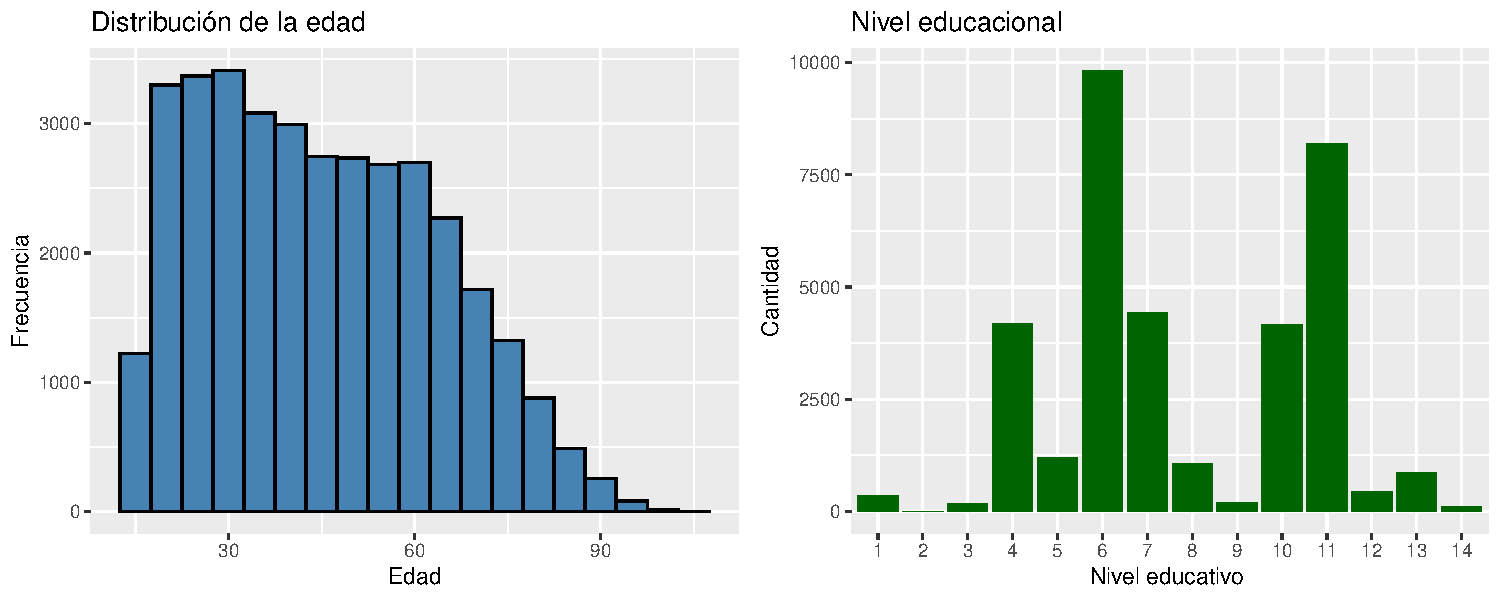
\includegraphics[keepaspectratio]{figs_pdf/edad-hist-edunivel-barra-1.pdf}}
Se observa una concentración significativa de registros entre los 25 y
los 40 años, donde las barras alcanzan su mayor altura, superando las
3.000 observaciones. A partir de ese rango, la frecuencia disminuye de
forma continua y progresiva hacia los grupos etarios superiores. El
declive después de los 40 indica una reducción natural de la fecundidad.

Mientras que en el segundo gráfico se observa que las categorías seis,
siete, ocho, nueve y diez presentan las barras más altas del gráfico,
siendo la número seis la que tiene la mayor altura. Estas barras se
destacan claramente por encima del resto. Por el contrario, las
categorías uno a cinco y once a catorce muestran barras
significativamente más bajas, con alturas similares entre ellas. Esto
indica que las observaciones están mayormente concentradas en los
niveles codificados entre el seis y el diez, mientras que los extremos
del rango, tanto iniciales como finales, tienen una menor frecuencia
relativa en comparación.

\newpage

\pandocbounded{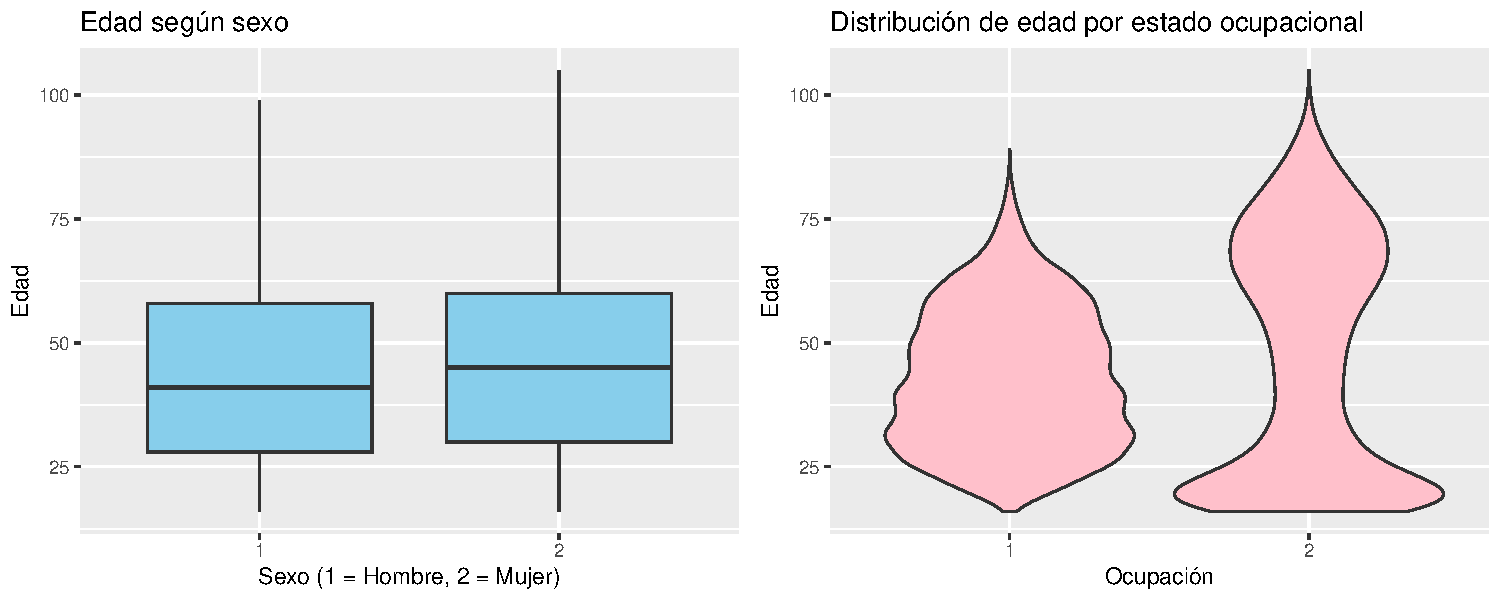
\includegraphics[keepaspectratio]{figs_pdf/edad-sexo-ocupacion-1.pdf}}

En el gráfico de caja , se observa que la distribución de la edad según
sexo presenta una mediana ligeramente mayor en las mujeres en
comparación con los hombres (código 1), lo que sugiere una mayor
proporción de mujeres en edades superiores dentro del conjunto
analizado. Esta diferencia también se evidencia en la dispersión, siendo
el rango intercuartílico y la presencia de valores extremos más amplios
en el caso femenino. Esta mayor heterogeneidad en la edad de las mujeres
puede estar asociada a fenómenos como la prolongación del ciclo
reproductivo en algunos subgrupos o una mayor longevidad estructural,
con implicancias en los análisis de fecundidad según cohortes.

Por otro lado, el gráfico de violín muestra la distribución de edad
según estado ocupacional. Aquí se distingue con claridad que el grupo
con ocupación 1, personas activas laboralmente, se concentra en edades
jóvenes y medias, principalmente entre los 25 y 50 años, con una
densidad mayor alrededor de los 35 años. En cambio, el grupo 2
,probablemente personas inactivas o fuera del mercado laboral---
presenta una distribución bimodal, con un primer pico en torno a los 30
años y un segundo en edades avanzadas (alrededor de los 65 a 75 años),
lo que podría corresponder a una combinación de personas en edad fértil
no insertas en el mercado laboral (por ejemplo, mujeres dedicadas al
trabajo doméstico o al cuidado) y personas jubiladas o en retiro.

\newpage

\pandocbounded{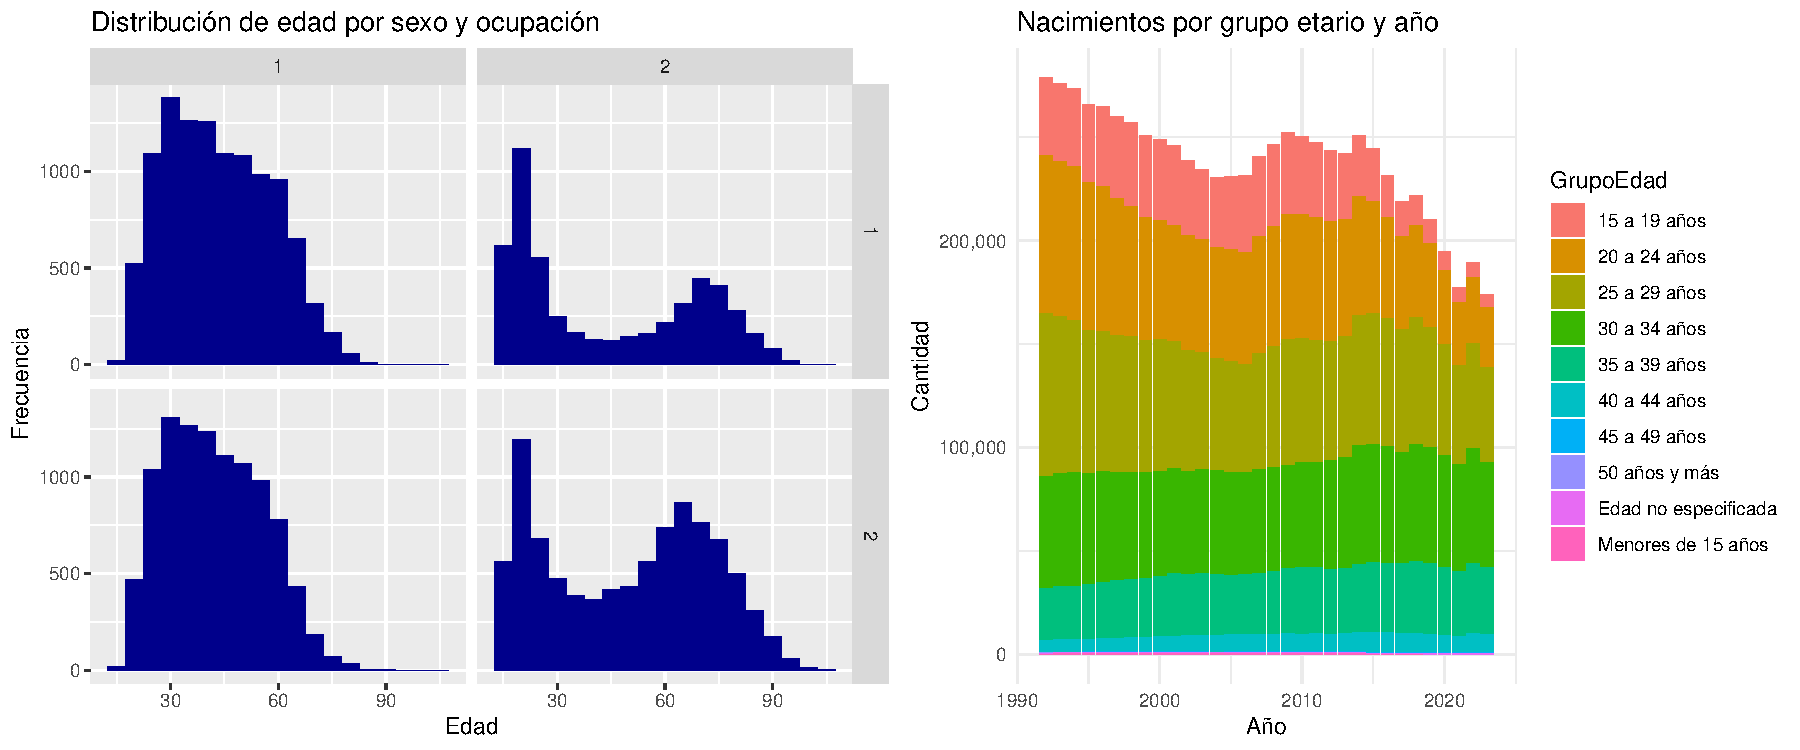
\includegraphics[keepaspectratio]{figs_pdf/facet-nacimientos-1.pdf}}

En primer lugar, los histogramas de la izquierda muestran que la mayoría
de las personas en edad reproductiva se concentran entre los 20 y 40
años, siendo este rango etario especialmente denso entre quienes se
encuentran ocupados laboralmente. En contraste, en los segmentos sin
ocupación formal (ocupación 2), se observa una mayor representación de
personas mayores, especialmente mujeres, lo que sugiere una fuerte
relación entre participación laboral, edad y potencial reproductivo.
Esta estructura etaria evidencia un desplazamiento de la fuerza
reproductiva hacia edades más avanzadas, en un contexto de transición
demográfica y envejecimiento poblacional.

Complementariamente, el gráfico de barras apiladas sobre nacimientos por
grupo etario de la madre y año refuerza esta tendencia, mostrando una
marcada disminución en la fecundidad global desde los años 2000 en
adelante, con una caída aún más pronunciada a partir de 2015. A nivel
etario, se aprecia una reducción sostenida en los nacimientos
provenientes de mujeres menores de 20 años, especialmente en el grupo de
15 a 19 años, lo que indica una baja en la fecundidad adolescente,
posiblemente atribuible a mayores niveles educativos, acceso a métodos
anticonceptivos y cambios en las expectativas reproductivas.
Paralelamente, se observa un leve pero consistente incremento relativo
en los nacimientos en mujeres de 30 años y más, particularmente en los
tramos de 30 a 34 y 35 a 39 años, lo que sugiere un patrón de
postergación de la maternidad.

\newpage

\section{Técnica de selección}\label{tuxe9cnica-de-selecciuxf3n}

Para complementar el análisis exploratorio de fecundidad y apoyar la
toma de decisiones, se aplicó un \textbf{árbol de decisión} como técnica
analítica avanzada, ya que es una pieza clave del Business Intelligence,
permitiendo modelar relaciones complejas entre variables de manera
interpretable (Curto Díaz \& Conesa, 2011). Esta metodología fue
seleccionada debido a su capacidad para modelar relaciones complejas
entre variables de forma visual, sencilla e interpretable (Breiman et
al.,1984), los árboles de decisión son especialmente útiles en problemas
de clasificación donde la interpretabilidad es crítica para la toma de
decisiones estratégicas.

El árbol de decisión clasifica las observaciones mediante divisiones
binarias sucesivas que maximizan la pureza de los nodos resultantes. En
este proyecto, se utilizó para identificar combinaciones de
características socioeconómicas (edad, nivel educativo, ingreso,
ocupación, etc.) que predicen la pertenencia a un grupo con mayor o
menor probabilidad de fecundidad o a grupos etarios críticos.

Otras técnicas consideradas incluyen:

\begin{itemize}
\tightlist
\item
  \textbf{Regresión logística:} aunque interpretable, esta técnica es
  menos flexible para capturar interacciones no lineales entre variables
  (Hastie et al., 2009).
\item
  \textbf{Redes neuronales:} aunque poderosas, estas técnicas son menos
  interpretables y requieren mayores recursos computacionales
  (Goodfellow et al., 2016).
\item
  \textbf{Clustering:} no es adecuado para problemas de clasificación
  supervisada como este (Kuhn \& Johnson, 2013).
\end{itemize}

Basándonos en estos criterios, el árbol de decisión fue seleccionado
como la técnica más adecuada para este análisis.

\subsection{\texorpdfstring{Validación Cruzada para la Selección del
Parámetro
\texttt{cp}}{Validación Cruzada para la Selección del Parámetro cp}}\label{validaciuxf3n-cruzada-para-la-selecciuxf3n-del-paruxe1metro-cp}

Para asegurar que el árbol de decisión fuera robusto y evitara
sobreajuste, se aplicó un proceso de \textbf{validación cruzada} durante
la selección del parámetro de complejidad (\texttt{cp}). El árbol
inicial se entrenó con un valor muy bajo de \texttt{cp}
(\texttt{cp\ =\ 0.0001}) para explorar todas las posibles divisiones.
Posteriormente, se utilizó la \textbf{regla 1-SE}, que selecciona el
árbol más simple (mayor \texttt{cp}) cuyo error no excede en más de una
desviación estándar el error mínimo. Esta metodología garantizó que el
árbol final fuera interpretable y generalizara adecuadamente a nuevos
datos (James et al., 2021).

El proceso de validación cruzada se realizó internamente mediante la
función \texttt{rpart}, que genera una tabla de errores de validación
cruzada (\texttt{cptable}). Esta tabla contiene el error de validación
(\texttt{xerror}) para diferentes valores de \texttt{cp}. La regla 1-SE
selecciona el árbol más simple (mayor \texttt{cp}) cuyo error no excede
en más de una desviación estándar (\texttt{xstd}) el error mínimo. Esto
asegura que el modelo sea lo suficientemente simple para evitar
sobreajuste (Kuhn \& Johnson, 2013).

\newpage

\subsection{Preparación de los Datos}\label{preparaciuxf3n-de-los-datos}

Se cargaron los datos desde el archivo Basefinal.xlsx utilizando la
función read\_excel del paquete \texttt{readxl}. Se realizaron
transformaciones iniciales, como la conversión de ingresos de texto a
valores numéricos \texttt{(gsub(",",\ ".",\ ing\_disp\_hog\_hd\_pc))}y
la eliminación de registros incompletos o con valores atípicos extremos.
Se creó una variable grupo\_hijos para clasificar a los hogares según el
número de hijos (0 hijos, 1--2 hijos, 3+ hijos). Partición de Datos: Los
datos se dividieron en conjuntos de entrenamiento (70\%) y prueba (30\%)
utilizando la función createDataPartition del paquete caret. Esta
partición fue estratificada según la variable dependiente (grupo\_hijos)
para asegurar una distribución equilibrada. Entrenamiento del Modelo: Se
entrenó un árbol de decisión utilizando la función rpart del paquete
rpart. Se utilizó un valor muy bajo de cp (cp = 0.0001) para explorar
todas las posibles divisiones. Se aplicó la regla 1-SE para seleccionar
el valor óptimo de cp basado en el error de validación cruzada
(cptable). Generación de Visualizaciones: Se generó un gráfico del árbol
podado utilizando la función rpart.plot. Se calculó la importancia de
las variables utilizando el atributo variable.importance del modelo
entrenado.

\subsection{Resultados e
interpretación}\label{resultados-e-interpretaciuxf3n}

\pandocbounded{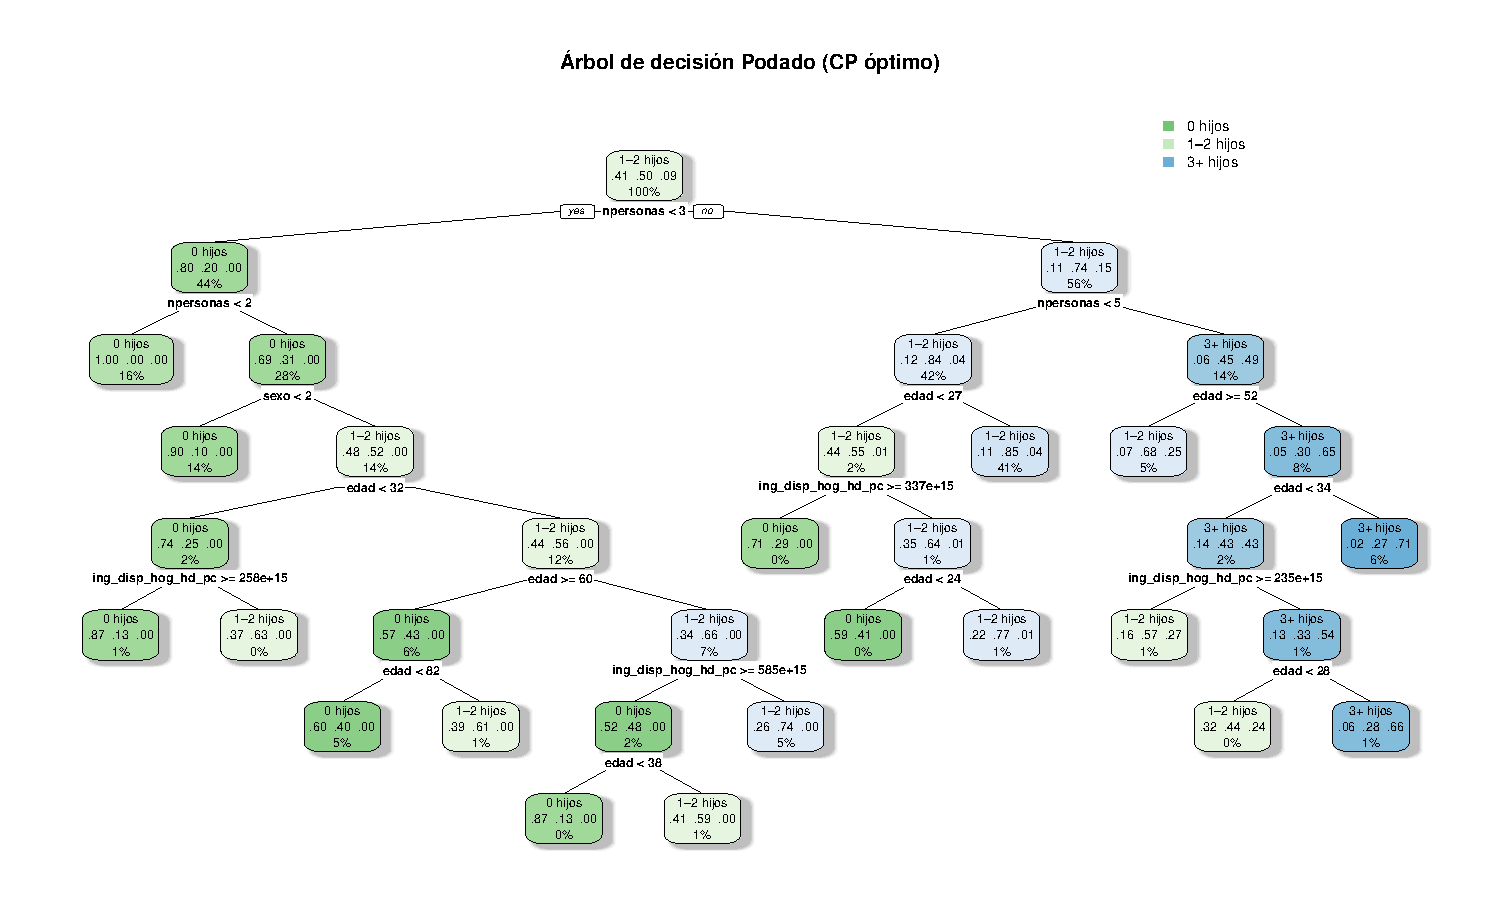
\includegraphics[keepaspectratio]{figs_pdf/arbol-podado-plot-1.pdf}}

El árbol de decisión muestra que las personas que viven en hogares
pequeños, especialmente de una o dos personas, tienden principalmente a
no tener hijos. A medida que el tamaño del hogar aumenta, también lo
hace la proporción de personas con uno o dos hijos, y en algunos casos
con tres o más. La edad influye de forma segmentada: las personas
menores de 34 años con ingresos bajos presentan mayores proporciones de
tres o más hijos, mientras que en los tramos de edad más avanzada
predominan los hogares sin hijos. El ingreso per cápita actúa como un
punto de quiebre dentro de los grupos con hijos: mayores ingresos se
asocian a una mayor proporción de personas sin hijos o con solo uno o
dos. La mayor parte de los nodos donde predominan las personas con tres
o más hijos aparece cuando se combinan bajos ingresos, edades entre 28 y
52 años, y hogares más grandes. El sexo tiene un efecto menor y acotado
a ramas específicas del árbol. En general, el patrón que emerge refleja
que los hogares pequeños, con edades más avanzadas o mayores ingresos,
se concentran en perfiles sin hijos, mientras que los hogares numerosos,
con edades medias y menores ingresos, se asocian con mayor número de
hijos.

\pandocbounded{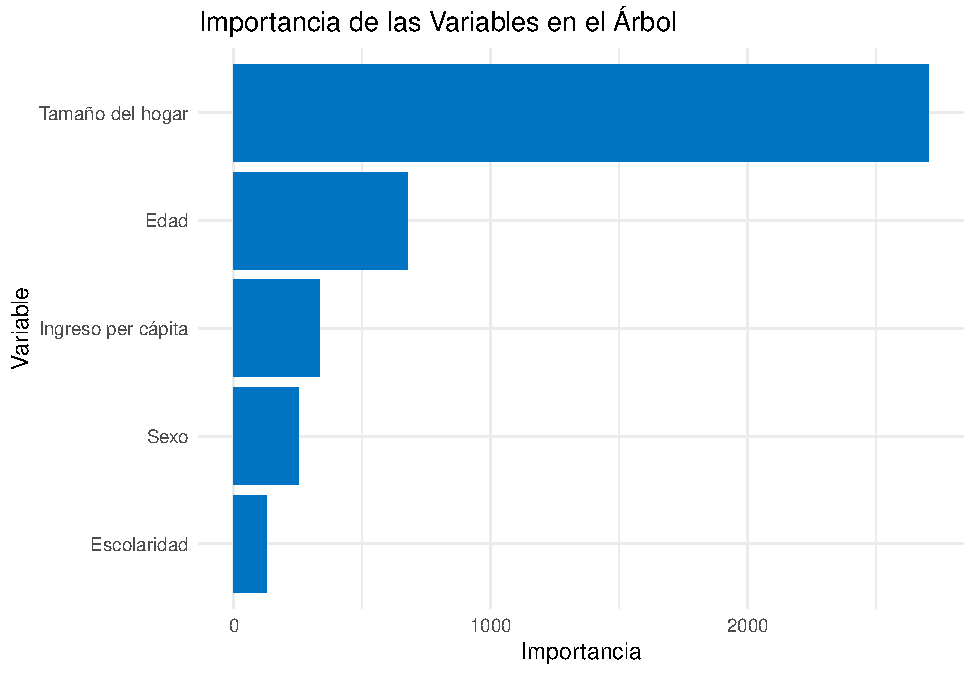
\includegraphics[keepaspectratio]{figs_pdf/unnamed-chunk-2-1.pdf}}

El gráfico de importancia de las variables del árbol muestra que el
tamaño del hogar es la variable más relevante para predecir la
fecundidad, lo que indica que el número de personas en un hogar tiene un
impacto significativo en la propensión a tener hijos. Esto sugiere que
hogares más grandes tienden a estar asociados con familias que tienen
más hijos, mientras que hogares pequeños están más relacionados con la
ausencia de hijos o familias con pocos hijos. En segundo lugar, la edad
es una variable clave, ya que los patrones de fecundidad varían
considerablemente con la etapa de vida: mujeres jóvenes (especialmente
entre 20 y 34 años) muestran tasas de fecundidad más altas, mientras que
en edades avanzadas la fecundidad disminuye drásticamente. La tercera
variable más importante es el ingreso per cápita , que actúa como un
factor determinante en la decisión de tener hijos. Menores ingresos se
asocian con una mayor probabilidad de tener tres o más hijos,
especialmente en combinación con edades medias y hogares más grandes,
mientras que mayores ingresos están vinculados a hogares sin hijos o con
uno o dos hijos. El sexo tiene una importancia moderada pero limitada a
ciertas ramas del árbol, lo que refleja su menor influencia directa en
comparación con otras variables. Finalmente, la escolaridad tiene la
menor relevancia en el modelo, lo que podría deberse a que su efecto
está mediado por factores como el ingreso o la edad. En conjunto, estos
resultados indican que el tamaño del hogar, la edad y el ingreso son los
principales predictores de la fecundidad, destacando la interacción
entre condiciones socioeconómicas y demográficas en la dinámica
reproductiva. Esta información puede ser utilizada para diseñar
políticas públicas focalizadas, priorizando intervenciones en hogares
grandes, grupos de edad específicos y niveles de ingreso bajos para
abordar desafíos relacionados con la fecundidad y el crecimiento
poblacional.

\newpage

\subsection{Implementación}\label{implementaciuxf3n}

Para comenzar con el análisis, es necesario instalar el software R y el
entorno de desarrollo RStudio(link en el anexo), una vez instalado R y
RStudio, abra RStudio y ejecute el siguiente código para instalar los
paquetes requeridos:

Para asegurarse de que los paquetes están correctamente instalados,
cargue las bibliotecas con el siguiente código:

\begin{Shaded}
\begin{Highlighting}[]
\CommentTok{\# Lista de librerías necesarias}
\NormalTok{required\_packages }\OtherTok{\textless{}{-}} \FunctionTok{c}\NormalTok{(}
  \StringTok{"shiny"}\NormalTok{, }\StringTok{"shinydashboard"}\NormalTok{, }\StringTok{"readxl"}\NormalTok{, }\StringTok{"dplyr"}\NormalTok{, }\StringTok{"ggplot2"}\NormalTok{,}
  \StringTok{"reshape2"}\NormalTok{, }\StringTok{"plotly"}\NormalTok{, }\StringTok{"DT"}\NormalTok{, }\StringTok{"car"}\NormalTok{, }\StringTok{"caret"}\NormalTok{, }\StringTok{"tidyr"}\NormalTok{,}
  \StringTok{"sf"}\NormalTok{, }\StringTok{"leaflet"}\NormalTok{, }\StringTok{"scales"}\NormalTok{, }\StringTok{"rmarkdown"}\NormalTok{, }\StringTok{"readr"}\NormalTok{,}
  \StringTok{"knitr"}\NormalTok{, }\StringTok{"pagedown"}\NormalTok{, }\StringTok{"tinytex"}\NormalTok{, }\StringTok{"forcats"}\NormalTok{, }\StringTok{"patchwork"}\NormalTok{,}
  \StringTok{"rpart"}\NormalTok{, }\StringTok{"rpart.plot"}\NormalTok{, }\StringTok{"naniar"}
\NormalTok{)}

\CommentTok{\# Función para verificar e instalar librerías}
\NormalTok{install\_and\_load\_packages }\OtherTok{\textless{}{-}} \ControlFlowTok{function}\NormalTok{(packages) \{}
  \ControlFlowTok{for}\NormalTok{ (pkg }\ControlFlowTok{in}\NormalTok{ packages) \{}
    \ControlFlowTok{if}\NormalTok{ (}\SpecialCharTok{!}\FunctionTok{require}\NormalTok{(pkg, }\AttributeTok{character.only =} \ConstantTok{TRUE}\NormalTok{)) \{}
      \FunctionTok{message}\NormalTok{(}\FunctionTok{paste}\NormalTok{(}\StringTok{"Instalando el paquete:"}\NormalTok{, pkg))}
      \CommentTok{\# Intenta instalar desde CRAN o GitHub si es necesario}
      \CommentTok{\# Para paquetes de CRAN:}
      \FunctionTok{install.packages}\NormalTok{(pkg, }\AttributeTok{dependencies =} \ConstantTok{TRUE}\NormalTok{)}
      \CommentTok{\# Para paquetes específicos que no estén en CRAN (ej. desde GitHub):}
      \CommentTok{\# remotes::install\_github("usuario/repositorio")}

      \ControlFlowTok{if}\NormalTok{ (}\SpecialCharTok{!}\FunctionTok{require}\NormalTok{(pkg, }\AttributeTok{character.only =} \ConstantTok{TRUE}\NormalTok{)) \{}
        \FunctionTok{stop}\NormalTok{(}\FunctionTok{paste}\NormalTok{(}\StringTok{"Error: No se pudo instalar y cargar el paquete"}\NormalTok{, pkg, }\StringTok{". }
\StringTok{                   Por favor, instálelo manualmente."}\NormalTok{))}
\NormalTok{      \}}
\NormalTok{    \}}
\NormalTok{  \}}
  \FunctionTok{message}\NormalTok{(}\StringTok{"Todos los paquetes requeridos están instalados y cargados."}\NormalTok{)}
\NormalTok{\}}

\CommentTok{\# Ejecutar la verificación e instalación}
\FunctionTok{install\_and\_load\_packages}\NormalTok{(required\_packages)}
\end{Highlighting}
\end{Shaded}

Proseguimos con la estructura de nuestro programa para el arbol de
decisión:

\begin{Shaded}
\begin{Highlighting}[]
\CommentTok{\# Carga de librerías necesarias para manipulación de datos, modelamiento y }
\CommentTok{\# visualización}
\FunctionTok{library}\NormalTok{(readxl)}
\FunctionTok{library}\NormalTok{(readr)}
\FunctionTok{library}\NormalTok{(dplyr)}
\FunctionTok{library}\NormalTok{(tidyr)}
\FunctionTok{library}\NormalTok{(rpart)}
\FunctionTok{library}\NormalTok{(rpart.plot)}
\FunctionTok{library}\NormalTok{(caret)}
\FunctionTok{library}\NormalTok{(car)}
\FunctionTok{library}\NormalTok{(ggplot2)}

\CommentTok{\# Lectura del archivo CSV que contiene los datos de personas de la encuesta EPF}
\NormalTok{epf }\OtherTok{\textless{}{-}} \FunctionTok{read\_delim}\NormalTok{(}\StringTok{"C:/Users/cesar/OneDrive/Escritorio/TrabajoFecundidadyHogares/Dashboard/epf\_persona.csv"}\NormalTok{, }\AttributeTok{delim =} \StringTok{";"}\NormalTok{,}
                  \AttributeTok{escape\_double =} \ConstantTok{FALSE}\NormalTok{, }\AttributeTok{trim\_ws =} \ConstantTok{TRUE}\NormalTok{)}

\CommentTok{\# Filtrado de jefes/as de hogar y selección de variables relevantes para e}
\CommentTok{\# el análisis}
\NormalTok{hogar\_base }\OtherTok{\textless{}{-}}\NormalTok{ epf }\SpecialCharTok{\%\textgreater{}\%}
  \FunctionTok{filter}\NormalTok{(sprincipal }\SpecialCharTok{==} \DecValTok{1}\NormalTok{) }\SpecialCharTok{\%\textgreater{}\%}
  \FunctionTok{select}\NormalTok{(folio, ing\_disp\_hog\_hd\_pc, edad, sexo, edue, edunivel,}
\NormalTok{         npersonas, cse, macrozona, estrato\_muestreo, ecivil)}

\CommentTok{\# Cálculo del número de hijos por hogar en base a los códigos de parentesco}
\NormalTok{hijos\_por\_folio }\OtherTok{\textless{}{-}}\NormalTok{ epf }\SpecialCharTok{\%\textgreater{}\%}
  \FunctionTok{filter}\NormalTok{(parentesco }\SpecialCharTok{\%in\%} \FunctionTok{c}\NormalTok{(}\DecValTok{3}\NormalTok{, }\DecValTok{4}\NormalTok{, }\DecValTok{5}\NormalTok{)) }\SpecialCharTok{\%\textgreater{}\%}
  \FunctionTok{group\_by}\NormalTok{(folio) }\SpecialCharTok{\%\textgreater{}\%}
  \FunctionTok{summarise}\NormalTok{(}\AttributeTok{num\_hijos =} \FunctionTok{n}\NormalTok{(), }\AttributeTok{.groups =} \StringTok{"drop"}\NormalTok{)}

\CommentTok{\# Unión de los datos de hogar con la cantidad de hijos y creación de variables }
\CommentTok{\# de modelamiento}
\NormalTok{hogares\_model }\OtherTok{\textless{}{-}}\NormalTok{ hogar\_base }\SpecialCharTok{\%\textgreater{}\%}
  \FunctionTok{left\_join}\NormalTok{(hijos\_por\_folio, }\AttributeTok{by =} \StringTok{"folio"}\NormalTok{) }\SpecialCharTok{\%\textgreater{}\%}
  \FunctionTok{mutate}\NormalTok{(}
    \AttributeTok{num\_hijos =} \FunctionTok{replace\_na}\NormalTok{(num\_hijos, }\DecValTok{0}\NormalTok{),}
    \AttributeTok{tiene\_hijos =} \FunctionTok{ifelse}\NormalTok{(num\_hijos }\SpecialCharTok{\textgreater{}} \DecValTok{0}\NormalTok{, }\DecValTok{1}\NormalTok{, }\DecValTok{0}\NormalTok{),}
    \AttributeTok{ing\_disp\_hog\_hd\_pc =} \FunctionTok{as.numeric}\NormalTok{(}\FunctionTok{gsub}\NormalTok{(}\StringTok{","}\NormalTok{, }\StringTok{"."}\NormalTok{, ing\_disp\_hog\_hd\_pc)),}
    \AttributeTok{grupo\_hijos =} \FunctionTok{case\_when}\NormalTok{(}
\NormalTok{      num\_hijos }\SpecialCharTok{==} \DecValTok{0} \SpecialCharTok{\textasciitilde{}} \StringTok{"0 hijos"}\NormalTok{,}
\NormalTok{      num\_hijos }\SpecialCharTok{\%in\%} \DecValTok{1}\SpecialCharTok{:}\DecValTok{2} \SpecialCharTok{\textasciitilde{}} \StringTok{"1–2 hijos"}\NormalTok{,}
\NormalTok{      num\_hijos }\SpecialCharTok{\textgreater{}=} \DecValTok{3} \SpecialCharTok{\textasciitilde{}} \StringTok{"3+ hijos"}
\NormalTok{    ) }\SpecialCharTok{|\textgreater{}} \FunctionTok{factor}\NormalTok{(}\AttributeTok{levels =} \FunctionTok{c}\NormalTok{(}\StringTok{"0 hijos"}\NormalTok{, }\StringTok{"1–2 hijos"}\NormalTok{, }\StringTok{"3+ hijos"}\NormalTok{))}
\NormalTok{  )}

\CommentTok{\# División del conjunto de datos en entrenamiento (70\%) y prueba (30\%) de }
\CommentTok{\# forma estratificada}
\FunctionTok{set.seed}\NormalTok{(}\DecValTok{123}\NormalTok{)}
\NormalTok{trainIndex }\OtherTok{\textless{}{-}} \FunctionTok{createDataPartition}\NormalTok{(hogares\_model}\SpecialCharTok{$}\NormalTok{grupo\_hijos, }\AttributeTok{p =} \FloatTok{0.7}\NormalTok{, }\AttributeTok{list =} \ConstantTok{FALSE}\NormalTok{)}
\NormalTok{train\_data }\OtherTok{\textless{}{-}}\NormalTok{ hogares\_model[trainIndex, ]}
\NormalTok{test\_data  }\OtherTok{\textless{}{-}}\NormalTok{ hogares\_model[}\SpecialCharTok{{-}}\NormalTok{trainIndex, ]}

\CommentTok{\# Construcción del árbol de decisión completo para predecir grupo de hijos }
\CommentTok{\# según variables sociodemográficas}
\NormalTok{arbol\_completo }\OtherTok{\textless{}{-}} \FunctionTok{rpart}\NormalTok{(grupo\_hijos }\SpecialCharTok{\textasciitilde{}}\NormalTok{ npersonas }\SpecialCharTok{+}\NormalTok{ ing\_disp\_hog\_hd\_pc }\SpecialCharTok{+}\NormalTok{ edad }\SpecialCharTok{+}\NormalTok{ edue }\SpecialCharTok{+}\NormalTok{ sexo,}
                        \AttributeTok{data =}\NormalTok{ train\_data,}
                        \AttributeTok{method =} \StringTok{"class"}\NormalTok{,}
                        \AttributeTok{control =} \FunctionTok{rpart.control}\NormalTok{(}\AttributeTok{cp =} \FloatTok{0.0001}\NormalTok{))}

\CommentTok{\# Selección del parámetro de complejidad óptimo (cp) utilizando la regla 1{-}SE }
\CommentTok{\# para evitar sobreajuste}
\NormalTok{min\_xerror\_idx }\OtherTok{\textless{}{-}} \FunctionTok{which.min}\NormalTok{(arbol\_completo}\SpecialCharTok{$}\NormalTok{cptable[,}\StringTok{"xerror"}\NormalTok{])}
\NormalTok{min\_xerror }\OtherTok{\textless{}{-}}\NormalTok{ arbol\_completo}\SpecialCharTok{$}\NormalTok{cptable[min\_xerror\_idx,}\StringTok{"xerror"}\NormalTok{]}
\NormalTok{se\_xerror }\OtherTok{\textless{}{-}}\NormalTok{ arbol\_completo}\SpecialCharTok{$}\NormalTok{cptable[min\_xerror\_idx,}\StringTok{"xstd"}\NormalTok{]}

\NormalTok{cp\_1se\_rule }\OtherTok{\textless{}{-}}\NormalTok{ arbol\_completo}\SpecialCharTok{$}\NormalTok{cptable[}
\NormalTok{  arbol\_completo}\SpecialCharTok{$}\NormalTok{cptable[,}\StringTok{"xerror"}\NormalTok{] }\SpecialCharTok{\textless{}=}\NormalTok{ (min\_xerror }\SpecialCharTok{+}\NormalTok{ se\_xerror), }\StringTok{"CP"}
\NormalTok{]}

\NormalTok{cp\_1se\_rule }\OtherTok{\textless{}{-}} \FunctionTok{ifelse}\NormalTok{(}\FunctionTok{length}\NormalTok{(cp\_1se\_rule) }\SpecialCharTok{\textgreater{}} \DecValTok{0}\NormalTok{, }\FunctionTok{max}\NormalTok{(cp\_1se\_rule),}
\NormalTok{                      arbol\_completo}\SpecialCharTok{$}\NormalTok{cptable[min\_xerror\_idx,}\StringTok{"CP"}\NormalTok{])}

\CommentTok{\# Poda del árbol completo utilizando el cp óptimo calculado anteriormente}
\NormalTok{arbol\_podado\_optimo }\OtherTok{\textless{}{-}} \FunctionTok{prune}\NormalTok{(arbol\_completo, }\AttributeTok{cp =}\NormalTok{ cp\_1se\_rule)}

\CommentTok{\# Visualización del árbol de decisión final podado, con etiquetas informativas}
\CommentTok{\# y diseño personalizado}
\FunctionTok{invisible}\NormalTok{(}\FunctionTok{rpart.plot}\NormalTok{(arbol\_podado\_optimo,}
           \AttributeTok{type =} \DecValTok{2}\NormalTok{,}
           \AttributeTok{extra =} \DecValTok{104}\NormalTok{,}
           \AttributeTok{fallen.leaves =} \ConstantTok{FALSE}\NormalTok{,}
           \AttributeTok{box.palette =} \StringTok{"GnBu"}\NormalTok{,}
           \AttributeTok{shadow.col =} \StringTok{"gray"}\NormalTok{,}
           \AttributeTok{main =} \StringTok{"Árbol de decisión Podado (CP óptimo)"}\NormalTok{))}
\end{Highlighting}
\end{Shaded}

Corroboramos con el siguiente programa la importancia de variables a
tener en consideración.

\begin{Shaded}
\begin{Highlighting}[]
\CommentTok{\# Se cargan las librerías necesarias para manipulación de datos, modelado y }
\CommentTok{\#visualización.}
\FunctionTok{library}\NormalTok{(readxl)  }
\FunctionTok{library}\NormalTok{(readr)   }
\FunctionTok{library}\NormalTok{(dplyr)   }
\FunctionTok{library}\NormalTok{(tidyr)   }
\FunctionTok{library}\NormalTok{(rpart)   }
\FunctionTok{library}\NormalTok{(rpart.plot) }
\FunctionTok{library}\NormalTok{(caret)   }
\FunctionTok{library}\NormalTok{(ggplot2) }
\FunctionTok{library}\NormalTok{(naniar) }
\FunctionTok{library}\NormalTok{(knitr)   }
\FunctionTok{library}\NormalTok{(kableExtra)  }

\CommentTok{\# {-}{-}{-} CARGA DE DATOS {-}{-}{-}}
\NormalTok{epf }\OtherTok{\textless{}{-}} \FunctionTok{read\_delim}\NormalTok{(}\StringTok{"C:/Users/cesar/OneDrive/Escritorio/TrabajoFecundidadyHogares/Dashboard/epf\_persona.csv"}\NormalTok{, }\AttributeTok{delim =} \StringTok{";"}\NormalTok{, }
                  \AttributeTok{escape\_double =} \ConstantTok{FALSE}\NormalTok{, }\AttributeTok{trim\_ws =} \ConstantTok{TRUE}\NormalTok{)}
\NormalTok{df\_variable }\OtherTok{\textless{}{-}} \FunctionTok{read\_excel}\NormalTok{(}\StringTok{"C:/Users/cesar/OneDrive/Escritorio/TrabajoFecundidadyHogares/Dashboard/Basefinal.xlsx"}\NormalTok{,}
                          \AttributeTok{sheet =} \StringTok{"epf"}\NormalTok{)}

\CommentTok{\# Se filtran los datos para quedarse solo con los jefes/as de hogar }
\CommentTok{\# (sprincipal == 1) y se seleccionan variables relevantes como ingreso, edad, }
\CommentTok{\#sexo, educación, tamaño del hogar, etc.}
\NormalTok{hogar\_base }\OtherTok{\textless{}{-}}\NormalTok{ epf }\SpecialCharTok{\%\textgreater{}\%}
  \FunctionTok{filter}\NormalTok{(sprincipal }\SpecialCharTok{==} \DecValTok{1}\NormalTok{) }\SpecialCharTok{\%\textgreater{}\%}
  \FunctionTok{select}\NormalTok{(}
\NormalTok{    folio, ing\_disp\_hog\_hd\_pc, edad, sexo, edue, edunivel,}
\NormalTok{    npersonas, cse, macrozona, estrato\_muestreo, ecivil}
\NormalTok{  )}

\CommentTok{\# Se calcula el número de hijos por hogar, identificando a los hijos mediante }
\CommentTok{\# el campo "parentesco".}
\NormalTok{hijos\_por\_folio }\OtherTok{\textless{}{-}}\NormalTok{ epf }\SpecialCharTok{\%\textgreater{}\%}
  \FunctionTok{filter}\NormalTok{(parentesco }\SpecialCharTok{\%in\%} \FunctionTok{c}\NormalTok{(}\DecValTok{3}\NormalTok{, }\DecValTok{4}\NormalTok{, }\DecValTok{5}\NormalTok{)) }\SpecialCharTok{\%\textgreater{}\%}
  \FunctionTok{group\_by}\NormalTok{(folio) }\SpecialCharTok{\%\textgreater{}\%}
  \FunctionTok{summarise}\NormalTok{(}\AttributeTok{num\_hijos =} \FunctionTok{n}\NormalTok{(), }\AttributeTok{.groups =} \StringTok{"drop"}\NormalTok{)}

\CommentTok{\# Se une la información de los hogares con el número de hijos calculado }
\CommentTok{\# anteriormente.}
\CommentTok{\# Se crean nuevas variables para facilitar el análisis:}
\CommentTok{\# {-} num\_hijos: número de hijos (0 si no hay hijos)}
\CommentTok{\# {-} tiene\_hijos: variable binaria (1 si tiene hijos, 0 si no)}
\CommentTok{\# {-} grupo\_hijos: clasificación de los hogares según el número de hijos (0 hijos,}
\CommentTok{\# 1{-}2 hijos, 3+ hijos)}
\NormalTok{hogares\_model }\OtherTok{\textless{}{-}}\NormalTok{ hogar\_base }\SpecialCharTok{\%\textgreater{}\%}
  \FunctionTok{left\_join}\NormalTok{(hijos\_por\_folio, }\AttributeTok{by =} \StringTok{"folio"}\NormalTok{) }\SpecialCharTok{\%\textgreater{}\%}
  \FunctionTok{mutate}\NormalTok{(}
    \AttributeTok{num\_hijos =} \FunctionTok{replace\_na}\NormalTok{(num\_hijos, }\DecValTok{0}\NormalTok{),}
    \AttributeTok{tiene\_hijos =} \FunctionTok{ifelse}\NormalTok{(num\_hijos }\SpecialCharTok{\textgreater{}} \DecValTok{0}\NormalTok{, }\DecValTok{1}\NormalTok{, }\DecValTok{0}\NormalTok{),}
    \AttributeTok{ing\_disp\_hog\_hd\_pc =} \FunctionTok{as.numeric}\NormalTok{(}\FunctionTok{gsub}\NormalTok{(}\StringTok{","}\NormalTok{, }\StringTok{"."}\NormalTok{, ing\_disp\_hog\_hd\_pc)),}
    \AttributeTok{grupo\_hijos =} \FunctionTok{case\_when}\NormalTok{(}
\NormalTok{      num\_hijos }\SpecialCharTok{==} \DecValTok{0} \SpecialCharTok{\textasciitilde{}} \StringTok{"0 hijos"}\NormalTok{,}
\NormalTok{      num\_hijos }\SpecialCharTok{\%in\%} \DecValTok{1}\SpecialCharTok{:}\DecValTok{2} \SpecialCharTok{\textasciitilde{}} \StringTok{"1–2 hijos"}\NormalTok{,}
\NormalTok{      num\_hijos }\SpecialCharTok{\textgreater{}=} \DecValTok{3} \SpecialCharTok{\textasciitilde{}} \StringTok{"3+ hijos"}
\NormalTok{    ) }\SpecialCharTok{|\textgreater{}} \FunctionTok{factor}\NormalTok{(}\AttributeTok{levels =} \FunctionTok{c}\NormalTok{(}\StringTok{"0 hijos"}\NormalTok{, }\StringTok{"1–2 hijos"}\NormalTok{, }\StringTok{"3+ hijos"}\NormalTok{))}
\NormalTok{  )}

\CommentTok{\# {-}{-}{-} MODELO ÁRBOL DE DECISIÓN {-}{-}{-}}
\CommentTok{\# Se divide el conjunto de datos en entrenamiento (70\%) y prueba (30\%) de forma }
\CommentTok{\#estratificada.}
\FunctionTok{set.seed}\NormalTok{(}\DecValTok{123}\NormalTok{)  }\CommentTok{\# Para garantizar reproducibilidad}
\NormalTok{trainIndex }\OtherTok{\textless{}{-}} \FunctionTok{createDataPartition}\NormalTok{(hogares\_model}\SpecialCharTok{$}\NormalTok{grupo\_hijos, }\AttributeTok{p =} \FloatTok{0.7}\NormalTok{, }
                                  \AttributeTok{list =} \ConstantTok{FALSE}\NormalTok{)}
\NormalTok{train\_data }\OtherTok{\textless{}{-}}\NormalTok{ hogares\_model[trainIndex, ]}

\CommentTok{\# Se entrena un árbol de decisión completo para predecir el grupo de hijos }
\CommentTok{\# basado en variables sociodemográficas como tamaño del hogar, ingreso, edad, }
\CommentTok{\#escolaridad y sexo.}
\NormalTok{arbol\_completo }\OtherTok{\textless{}{-}} \FunctionTok{rpart}\NormalTok{(grupo\_hijos }\SpecialCharTok{\textasciitilde{}}\NormalTok{ npersonas }\SpecialCharTok{+}\NormalTok{ ing\_disp\_hog\_hd\_pc }\SpecialCharTok{+}\NormalTok{ edad }\SpecialCharTok{+} 
\NormalTok{                          edue }\SpecialCharTok{+}\NormalTok{ sexo,}
                        \AttributeTok{data =}\NormalTok{ train\_data,}
                        \AttributeTok{method =} \StringTok{"class"}\NormalTok{,}
                        \AttributeTok{control =} \FunctionTok{rpart.control}\NormalTok{(}\AttributeTok{cp =} \FloatTok{0.0001}\NormalTok{))}

\CommentTok{\# Pruning del árbol utilizando la regla 1{-}SE para evitar sobreajuste.}
\CommentTok{\# Se selecciona el valor óptimo de cp (complejidad) basado en el error de }
\CommentTok{\# validación cruzada.}
\NormalTok{min\_xerror\_idx }\OtherTok{\textless{}{-}} \FunctionTok{which.min}\NormalTok{(arbol\_completo}\SpecialCharTok{$}\NormalTok{cptable[, }\StringTok{"xerror"}\NormalTok{])}
\NormalTok{min\_xerror }\OtherTok{\textless{}{-}}\NormalTok{ arbol\_completo}\SpecialCharTok{$}\NormalTok{cptable[min\_xerror\_idx, }\StringTok{"xerror"}\NormalTok{]}
\NormalTok{se\_xerror }\OtherTok{\textless{}{-}}\NormalTok{ arbol\_completo}\SpecialCharTok{$}\NormalTok{cptable[min\_xerror\_idx, }\StringTok{"xstd"}\NormalTok{]}

\NormalTok{cp\_1se\_rule }\OtherTok{\textless{}{-}}\NormalTok{ arbol\_completo}\SpecialCharTok{$}\NormalTok{cptable[}
\NormalTok{  arbol\_completo}\SpecialCharTok{$}\NormalTok{cptable[, }\StringTok{"xerror"}\NormalTok{] }\SpecialCharTok{\textless{}=}\NormalTok{ (min\_xerror }\SpecialCharTok{+}\NormalTok{ se\_xerror), }\StringTok{"CP"}
\NormalTok{]}

\NormalTok{cp\_1se }\OtherTok{\textless{}{-}} \FunctionTok{ifelse}\NormalTok{(}\FunctionTok{length}\NormalTok{(cp\_1se\_rule) }\SpecialCharTok{\textgreater{}} \DecValTok{0}\NormalTok{, }\FunctionTok{max}\NormalTok{(cp\_1se\_rule),}
\NormalTok{                 arbol\_completo}\SpecialCharTok{$}\NormalTok{cptable[min\_xerror\_idx, }\StringTok{"CP"}\NormalTok{])}

\CommentTok{\# Se poda el árbol utilizando el valor óptimo de cp encontrado.}
\NormalTok{arbol\_podado\_optimo }\OtherTok{\textless{}{-}} \FunctionTok{prune}\NormalTok{(arbol\_completo, }\AttributeTok{cp =}\NormalTok{ cp\_1se)}

\CommentTok{\# {-}{-}{-} IMPORTANCIA DE VARIABLES {-}{-}{-}}
\CommentTok{\# Se extrae la importancia de las variables del árbol podado.}
\NormalTok{importance\_df }\OtherTok{\textless{}{-}} \FunctionTok{data.frame}\NormalTok{(}
  \AttributeTok{Variable =} \FunctionTok{names}\NormalTok{(arbol\_podado\_optimo}\SpecialCharTok{$}\NormalTok{variable.importance),}
  \AttributeTok{Importance =} \FunctionTok{as.numeric}\NormalTok{(arbol\_podado\_optimo}\SpecialCharTok{$}\NormalTok{variable.importance)}
\NormalTok{)}

\CommentTok{\# Se renombran las variables para hacerlas más legibles en el gráfico.}
\NormalTok{nombres\_bonitos }\OtherTok{\textless{}{-}} \FunctionTok{c}\NormalTok{(}
  \AttributeTok{ing\_disp\_hog\_hd\_pc =} \StringTok{"Ingreso per cápita"}\NormalTok{,}
  \AttributeTok{npersonas =} \StringTok{"Tamaño del hogar"}\NormalTok{,}
  \AttributeTok{edue =} \StringTok{"Escolaridad"}\NormalTok{,}
  \AttributeTok{edad =} \StringTok{"Edad"}\NormalTok{,}
  \AttributeTok{sexo =} \StringTok{"Sexo"}
\NormalTok{)}

\NormalTok{importance\_df\_bonito }\OtherTok{\textless{}{-}}\NormalTok{ importance\_df }\SpecialCharTok{\%\textgreater{}\%}
  \FunctionTok{arrange}\NormalTok{(}\FunctionTok{desc}\NormalTok{(Importance)) }\SpecialCharTok{\%\textgreater{}\%}
  \FunctionTok{mutate}\NormalTok{(}\AttributeTok{Variable =}\NormalTok{ nombres\_bonitos[Variable])}

\CommentTok{\# {-}{-}{-} GRÁFICO DE IMPORTANCIA {-}{-}{-}}
\CommentTok{\# Se crea un gráfico de barras para visualizar la importancia de las variables }
\CommentTok{\#en el modelo.}
\FunctionTok{ggplot}\NormalTok{(importance\_df\_bonito, }\FunctionTok{aes}\NormalTok{(}\AttributeTok{x =} \FunctionTok{reorder}\NormalTok{(Variable, Importance),}
                                 \AttributeTok{y =}\NormalTok{ Importance)) }\SpecialCharTok{+}
  \FunctionTok{geom\_col}\NormalTok{(}\AttributeTok{fill =} \StringTok{"\#0073C2FF"}\NormalTok{) }\SpecialCharTok{+}
  \FunctionTok{coord\_flip}\NormalTok{() }\SpecialCharTok{+}
  \FunctionTok{labs}\NormalTok{(}\AttributeTok{title =} \StringTok{"Importancia de las Variables en el Árbol"}\NormalTok{,}
       \AttributeTok{x =} \StringTok{"Variable"}\NormalTok{,}
       \AttributeTok{y =} \StringTok{"Importancia"}\NormalTok{) }\SpecialCharTok{+}
  \FunctionTok{theme\_minimal}\NormalTok{()}
\end{Highlighting}
\end{Shaded}

\subsection{Consideraciones}\label{consideraciones}

El análisis de datos sociodemográficos para comprender patrones de
fecundidad implica el manejo de información sensible que requiere un
enfoque ético riguroso. A continuación, se destacan las principales
consideraciones éticas identificadas durante el desarrollo del proyecto:

Los datos utilizados provienen de fuentes públicas proporcionadas por el
INE, pero contienen variables sensibles como edad, ingreso per cápita,
estado civil, nivel educativo y parentesco . Para mitigar riesgos de
identificación individual, se implementaron medidas como la
anonimización de registros. Además, se creo una variable para trabajar
exclusivamente con los tipos de hogares según hijos, asegurando que el
análisis estuviera alineado con el objetivo estratégico del estudio.

Las recomendaciones derivadas del análisis podrían influir en políticas
públicas dirigidas a segmentos vulnerables de la población. Es
fundamental garantizar que estas intervenciones no estigmaticen a grupos
específicos (por ejemplo, familias numerosas o mujeres jóvenes) y que
promuevan la equidad en el acceso a recursos sociales.

El uso de un árbol de decisión permite una interpretación clara de los
resultados, lo que facilita la comunicación de hallazgos. Sin embargo,
es importante destacar que la interpretabilidad no elimina la necesidad
de validar continuamente los supuestos del modelo y monitorear su
impacto en diferentes contextos sociales.

A pesar de los esfuerzos por garantizar la calidad y representatividad
de los datos, el análisis presenta ciertas limitaciones que deben
considerarse al interpretar los resultados:

Supuestos del Modelo : el árbol de decisión asume relaciones no lineales
entre variables, pero no captura interacciones complejas que podrían
modelarse mejor con técnicas avanzadas como redes neuronales. Sin
embargo, estas últimas son menos interpretables y no se alinean con el
objetivo estratégico de claridad en la toma de decisiones. Poda del
Árbol : la aplicación de la regla 1-SE para seleccionar el parámetro de
complejidad (cp) busca evitar el sobreajuste, pero también puede
simplificar excesivamente el modelo, omitiendo patrones relevantes en
los datos.

Los datos cubren el periodo 2021-2022, lo que incluye cambios
significativos en las dinámicas sociales y económicas de Chile. Aunque
esto permite analizar tendencias a largo plazo, algunos patrones
recientes podrían estar subrepresentados.

Factores como acceso a servicios de salud, disponibilidad de métodos
anticonceptivos y apoyo social no están explícitamente incluidos en el
análisis, lo que podría sesgar las conclusiones sobre los determinantes
de la fecundidad.

Los hallazgos del modelo son específicos y pueden no ser aplicables a
otros países con diferentes dinámicas socioeconómicas. Además, el
análisis se centra las categorias de hogares según hijos.

Las recomendaciones propuestas, como priorizar programas de apoyo en
hogares con bajos ingresos y edades reproductivas, requieren recursos
sostenibles para su implementación. Sin una planificación adecuada,
existe el riesgo de que las intervenciones no logren los objetivos
esperados o generen dependencia estructural.

\subsection{Referencias}\label{referencias}

\begin{itemize}
\tightlist
\item
  Breiman, L., Friedman, J., Stone, C. J., \& Olshen, R. A. (1984).
  \emph{Classification and Regression Trees}. Chapman \& Hall/CRC.
\item
  Goodfellow, I., Bengio, Y., \& Courville, A. (2016). \emph{Deep
  Learning}. MIT Press.
\item
  Hastie, T., Tibshirani, R., \& Friedman, J. (2009). \emph{The Elements
  of Statistical Learning: Data Mining, Inference, and Prediction} (2nd
  ed.). Springer.
\item
  James, G., Witten, D., Hastie, T., \& Tibshirani, R. (2021). \emph{An
  Introduction to Statistical Learning: With Applications in R} (2nd
  ed.). Springer.
\item
  Kuhn, M., \& Johnson, K. (2013). \emph{Applied Predictive Modeling}.
  Springer. -Curto Díaz, J., Conesa, J. (2011) \emph{Introducción al
  Business Intelligence}. Editorial UOC
\end{itemize}

\subsection{ANEXO}\label{anexo}

\url{https://github.com/CesarSM04/Fecundidad_hogares}

\end{document}
